\documentclass[11pt,aspectratio=43,usenames,dvipsnames]{beamer}
\usepackage[utf8]{inputenc}
\usepackage{amsmath, amsfonts, amssymb, amsthm}
\usepackage[T1]{fontenc}
% mint: code chuck and syntax highlighting
%% outputdir should change according to pdf build directory
\usepackage[outputdir=build,cache=false]{minted}
\usepackage{lmodern}
\usepackage{xcolor}
\usepackage{setspace}
\usepackage{booktabs}
\usepackage{multirow}
\usepackage{graphicx}
\usepackage{fontawesome}

\usepackage[mode=tex]{standalone}
\usepackage{tikz}
\usetikzlibrary{decorations}
\usetikzlibrary{decorations.pathreplacing, intersections}
\usepackage{pgfplots}
\usetikzlibrary{calc,positioning}
\usepgfplotslibrary{fillbetween}
\pgfplotsset{compat=newest, scale only axis, width = 10cm}

% ---------------------------------------------------------------------
% Coordinate extraction
% #1: node name
% #2: output macro name: x coordinate
% #3: output macro name: y coordinate
\newcommand{\Getxycoords}[3]{%
    \pgfplotsextra{%
        % using `\pgfplotspointgetcoordinates' stores the (axis)
        % coordinates in `data point' which then can be called by
        % `\pgfkeysvalueof' or `\pgfkeysgetvalue'
        \pgfplotspointgetcoordinates{(#1)}%
        % `\global' (a TeX macro and not a TikZ/PGFPlots one) allows to
        % store the values globally
         \global\pgfkeysgetvalue{/data point/x}{#2}%
         \global\pgfkeysgetvalue{/data point/y}{#3}%
     }%
}
% ---------------------------------------------------------------------

\usepackage{ulem}
\usepackage{hyperref}
\usepackage{booktabs}
\usepackage{babel}
\usepackage{makecell}
\usepackage[para,online,flushleft]{threeparttable}
\usepackage{pdfpages}
\usepackage{tcolorbox}
\usepackage{bm}
\usepackage{appendixnumberbeamer}
\usepackage{natbib}
\usepackage{caption}
\captionsetup[figure]{labelformat=empty}% redefines the caption setup of the figures environment in the beamer class.
\usetheme[compress]{Boadilla}
\usecolortheme{default}
\useoutertheme{miniframes}
\usefonttheme[onlymath]{serif}

\newcommand{\jump}[2]{\hyperlink{#1}{\beamerbutton{#2}}}
\newcommand{\extjump}[2]{\href{#1}{\beamerbutton{#2}}}
\newcommand{\orange}[1]{\textcolor{orange}{#1}}
\newcommand{\red}[1]{\textcolor{red}{#1}}
\newcommand{\blue}[1]{\textcolor{blue}{#1}}
\newcommand{\green}[1]{\textcolor{OliveGreen}{#1}}

\renewcommand{\square}{\scalebox{0.7}{$\blacksquare$ \hspace{0.5em}}}
\setbeamertemplate{itemize item}{\raisebox{0.1em}{\scalebox{0.7}{$\blacksquare$}}}
\setbeamertemplate{itemize subitem}[circle]
\setbeamertemplate{itemize subsubitem}{--}
\setbeamercolor{itemize item}{fg=black}
\setbeamercolor{itemize subitem}{fg=black}
\setbeamercolor{itemize subsubitem}{fg=black}
\setbeamercolor{item projected}{bg=darkgray,fg=white}
\definecolor{blue}{rgb}{0.2, 0.2, 0.7}
\setbeamercolor{alerted text}{fg=blue}
\setbeamertemplate{enumerate items}[circle]


\setbeamertemplate{headline}{}

%==========================================
\let\olditemize=\itemize
\let\endolditemize=\enditemize
\renewenvironment{itemize}{\olditemize \itemsep1em}{\endolditemize}
\let\oldenumerate=\enumerate
\let\endoldenumerate=\endenumerate
\renewenvironment{enumerate}{\oldenumerate \itemsep1em}{ \endoldenumerate}

\DeclareMathOperator*{\argmax}{\arg\!\max}
\DeclareMathOperator*{\E}{\mathbb{E}}
\DeclareMathOperator*{\var}{\rm Var}
\DeclareMathOperator*{\cov}{\rm Cov}

\theoremstyle{definition}
\newtheorem{assume}{Assumption}
\newtheorem{lem}{Lemma}
\newtheorem{proposition}{Proposition}
\newtheorem{thm}{Theorem}
\newtheorem{corol}{Corollary}

\AtBeginSection[]{
  \begin{frame}[noframenumbering]
  \vfill
  \centering
  \begin{beamercolorbox}[sep=8pt,center,shadow=true,rounded=true]{title}
    \usebeamerfont{title}\insertsection\par%
  \end{beamercolorbox}
  \vfill
  \end{frame}
}

\begin{document}
    \title[Unit 10]{Unit 10 \\ Banks, Money and the Credit Market }
    \author[Hui-Jun Chen]{Hui-Jun Chen}
    \institute[OSU]{The Ohio State University}
    % \date{\today}
    \date{\today}
    \setbeamertemplate{navigation symbols}{}
    \setstretch{1.2}

%-------------------------------------------------------
{
%	\usebackgroundtemplate{\includegraphics[width=1\paperwidth]{../EveningSky_cropped_edit43_bright.jpg}}
    \begin{frame}
% \vspace{3em}
        \centering
%		{\footnotesize 	ECON 4002 Intermediate Macroeconomic Theory}
        \maketitle
% \vspace{-1.5em}
% \centering
% \includegraphics[width=0.55\linewidth]{Pictures/houses.jpeg}


    \end{frame}
}

% -------------------------------------------
\setbeamertemplate{headline}
{
\setbeamercolor{section in head/foot}{fg=black, bg=white}
\vskip1em \tiny \insertsectionnavigationhorizontal{1\paperwidth}{\hspace{0.50\paperwidth}}{}
}
%------------------------------------------

\section[Intro]{Introduction}
\label{sec:Intro}

\begin{frame}{Introduction \extjump{https://www.core-econ.org/the-economy/book/text/10.html}{Textbook}}
\label{slide:Introduction}
\begin{center}
\begin{quote}
    Economics is a choice between alternatives all the time. Those are the trade-offs.
\end{quote}
\hfill - Paul Samuelson

\begin{itemize}
    \item Food spoils, barrels leak, yet all trades take \alert{time}.
    \item Time is both the friend and the foe: depreciation \& appreciation
    \item \alert{Inter-temporal assets} allow agents to \alert{carry value over time}.
    \item What are inter-temporal assets?
    \begin{table}
        \footnotesize
        \begin{tabular}{r|lllll}
            Examples
                & Money
                & Capital
                & Bond / Debt
                & Social Security
                & Housing
            \\
            \hline
            Value $ \uparrow /\downarrow  $
                & $ \downarrow  $
                & $ \downarrow  $
                & $ \downarrow  $
                & $ \uparrow  $
                & $ \uparrow  $ (?)
            \\
            \hline
            Cause (?)
                & inflates
                & tech
                & default
                & age
                & develop
            \\
        \end{tabular}
        \caption{Examples of Intertemporal Assets}
    \end{table}
\end{itemize}

\end{center}
\end{frame}

\section[Time \faClockO]{Income, Borrowing and Saving}
\label{sec:Income__Borrowing_and_Saving}

\begin{frame}{Money, Income and Wealth}
\label{slide:Money__Income_and_Wealth}
    \begin{itemize}
        \item \textbf{Money}: medium of exchange, allow \alert{transfer} of purchasing power
        \begin{itemize}
            \item Whether a currency is \textbf{trust-worthy} is important
        \end{itemize}
        \item (Flow) \textbf{Income}: amount of money receive for a period of time
        \begin{itemize}
            \item wage bill, market earning, investment, gov transfer
        \end{itemize}
        \item (Stock) \textbf{Wealth}: inter-temporal assets carry values
        \begin{itemize}
            \item buildings, land, machinery, capital goods $ - $ debts $ + $ credit
        \end{itemize}
    \end{itemize}
\end{frame}

\begin{frame}{Other Key Concepts}
\label{slide:Other_Key_Concepts}
    \begin{itemize}
        \item Depreciation / Appreciation: value of stock $ \downarrow / \uparrow  $ over time
        \item Net income $ = $ gross income $ - $ depreciation
        \item Savings: income not consumed
        \item Investment: Expenditure on newly produced capital goods
    \end{itemize}
\end{frame}

\begin{frame}{Inter-temporal Substitution}
\label{slide:Inter_temporal_Substitution}
    \begin{itemize}
        \item As time is here, \alert{current you} and \alert{future you} are sharing for resources
        \item The opportunity cost of \alert{more current goods} is \alert{less future gooes}
        \item \textbf{Borrowing} and \textbf{lending} allows resource-sharing across time
        \item The ``price'' for inter-temporal substitution depends on the assets;
        \item In the case of borrowing / lending, we call the ``price'' as \textbf{interest rate}
        \item The position matters: the impact of change in interest rate depends on whether you are \alert{borrower} or \alert{lender}
    \end{itemize}
\end{frame}

\begin{frame}{Borrowing}
\label{slide:Borrowing}
    \begin{columns}
        \begin{column}{0.5\textwidth}
            \only<1>{
            \begin{itemize}
                \item Julia has $ 100 $ endowment in the \alert{future}: Nothing for today. \faFrownO
                \item Julia wants to \alert{borrow} some consumption \alert{today} and promise to repay \alert{tomorrow} with her endowment
                \item How \alert{much} goods could Julia get for today if she commit all her endowment tomorrow?
            \end{itemize}
            }
            \only<2>{
            \begin{itemize}
                \item \textbf{Interest rate ($r$)}: price to bring purchasing power forward in time
                \item current $ \underbrace{\Longrightarrow}_{1+r} $ future
                \item
                \begin{tabular}{cc}
                    today
                        & tomorrow
                    \\
                    1
                        & $ 1+r $
                    \\
                    $ \frac{1}{1+r} $
                        & 1
                    \\
                \end{tabular}
                \item Slope: $ \frac{1}{1+r} $, since future $ C $ on $ y $-axis and current on $ x $-axis
            \end{itemize}
            }
            \only<3>{
            \begin{itemize}
                \item $ (1+r) $: \textbf{supply-side} tradeoff $ \Rightarrow  $ MRT
                \item Motivation for borrowing \& lending:
                \begin{enumerate}
                    \item \alert{consumption smoothing} (Julia's case)
                    \item \alert{Impatience}
                \end{enumerate}


            \end{itemize}
            }
        \end{column}
        \begin{column}{0.5\textwidth}
            \begin{figure}
                \centering
                \only<1-2>{
                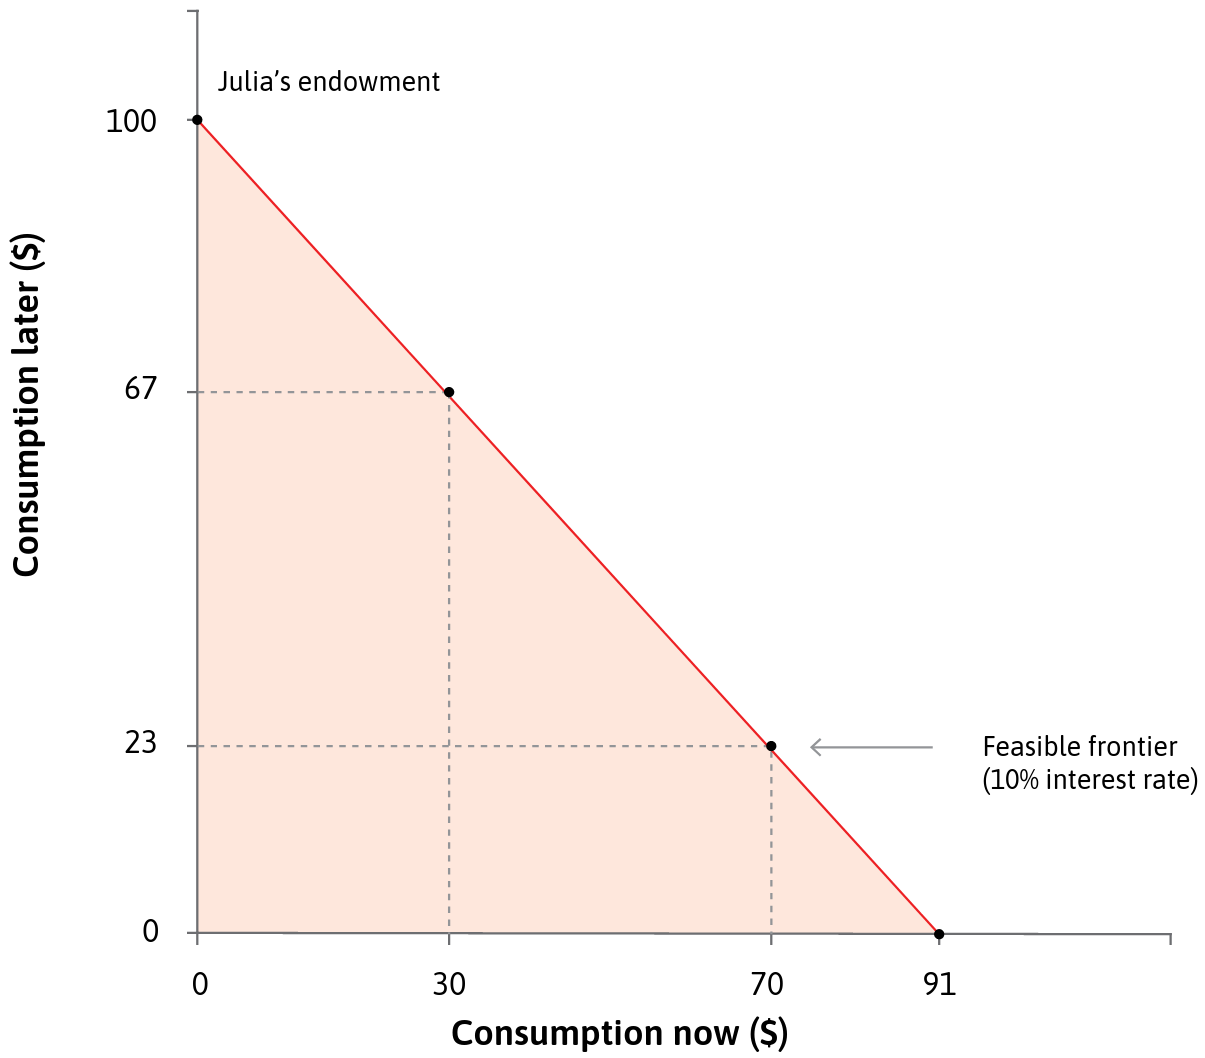
\includegraphics[width=\textwidth]{./figures/Figure1.png}
                }
                \only<3>{
                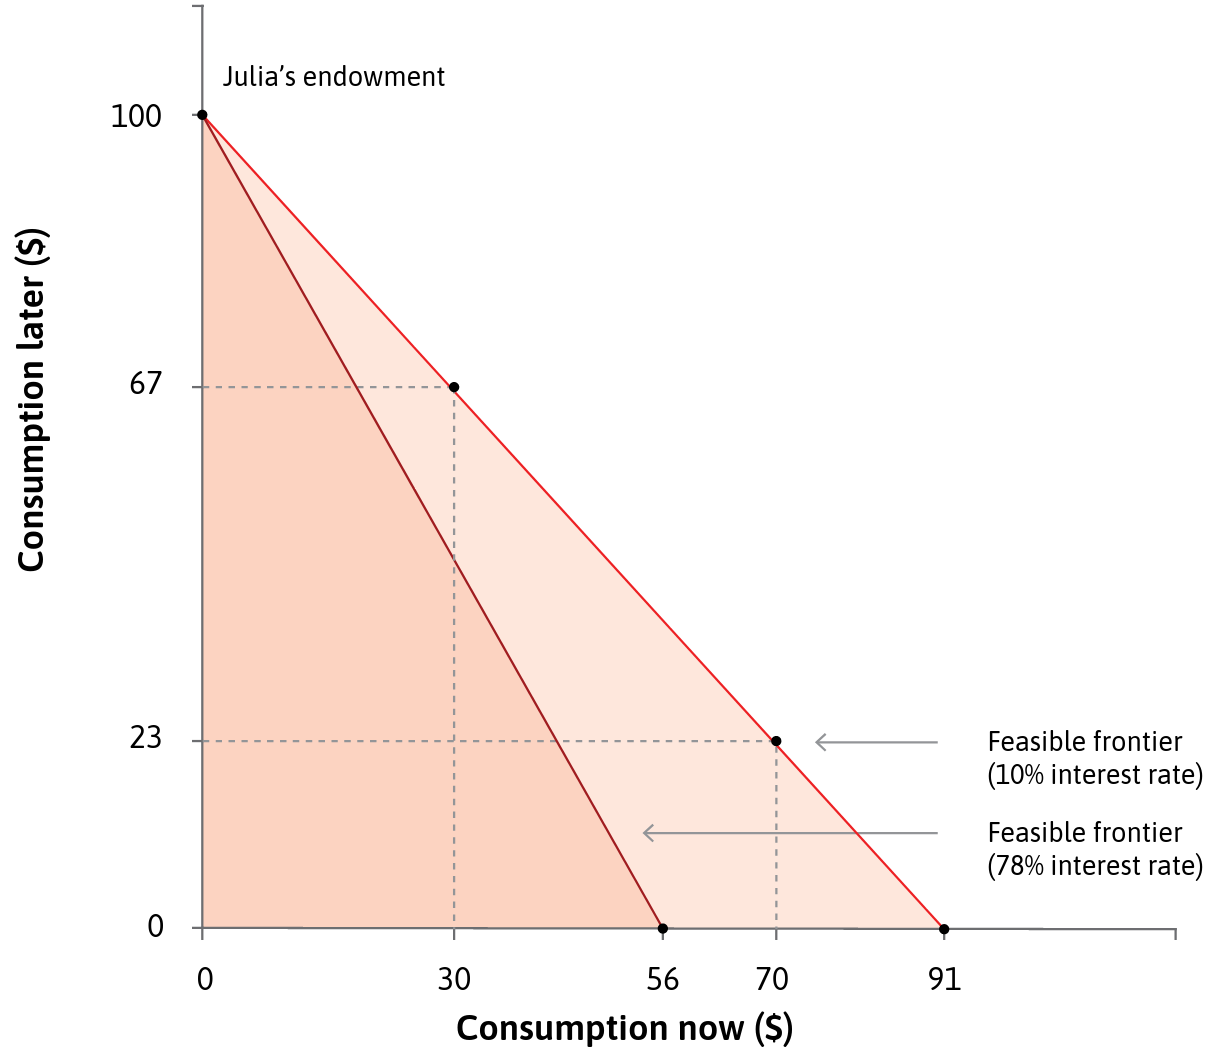
\includegraphics[width=\textwidth]{./figures/Figure2.png}
                }
            \end{figure}
        \end{column}
    \end{columns}
\end{frame}

\begin{frame}{Consumption Smoothing}
\label{slide:Consumption_Smoothing}
    \begin{columns}
        \begin{column}{0.5\textwidth}
            \begin{itemize}
                \item The indifference curve exhibits \textbf{diminishing marginal returns to consumption} in one period.
                \item \alert{Avoid consuming a lot in one period and little in the other.}
                \item \textbf{Discount rate ($ \rho $)}: measure of one's impatience/precautions
            \end{itemize}
        \end{column}
        \begin{column}{0.5\textwidth}
            \begin{figure}
                \centering
                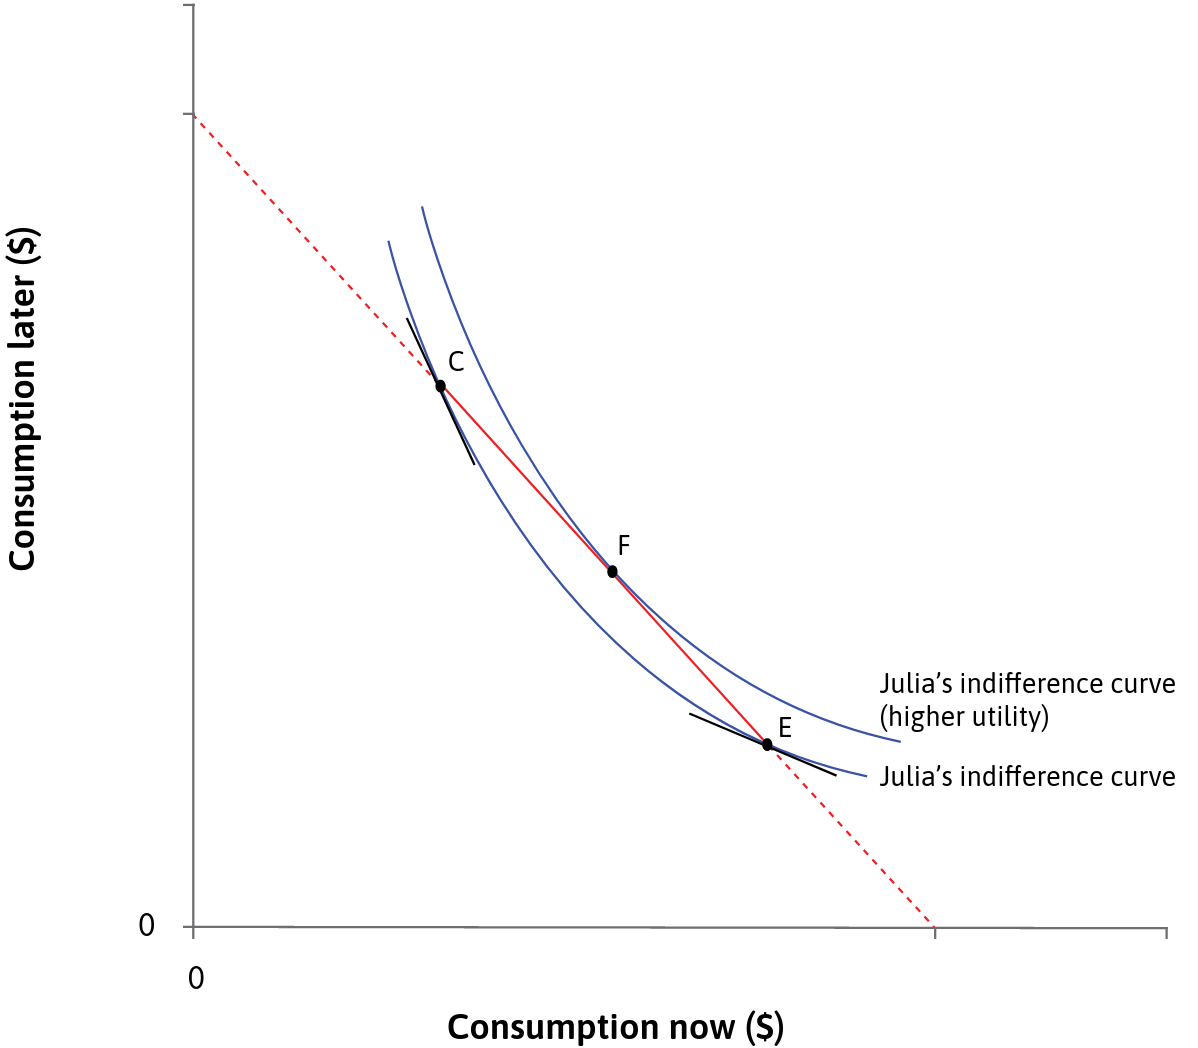
\includegraphics[width=\textwidth]{./figures/Figure3.png}
            \end{figure}

        \end{column}
    \end{columns}
\end{frame}

\begin{frame}{Pure Impatience}
\label{slide:Pure_Impatience}

        \begin{center}
            \textit{How much more do you value a good now than later?}
        \end{center}

        \vspace{1em}

    \begin{itemize}
        \item Consumption smoothing may appear as being impatient.
        \item However, we differentiate it from pure impatience = being impatient as a person.
        \begin{itemize}
            \item \textbf{Myopia} (short-sightedness): People experience the present satisfaction more strongly than the same satisfaction later
            \item \textbf{Prudence}: People know that they may not be around in the future, and so they want to consume now
        \end{itemize}


    \end{itemize}
\end{frame}

\begin{frame}{Optimal Decision-Making}
\label{slide:Optimal_Decision_Making}
    \begin{columns}
        \begin{column}{0.5\textwidth}

        \end{column}
        \begin{column}{0.5\textwidth}
            \begin{figure}
                \centering
                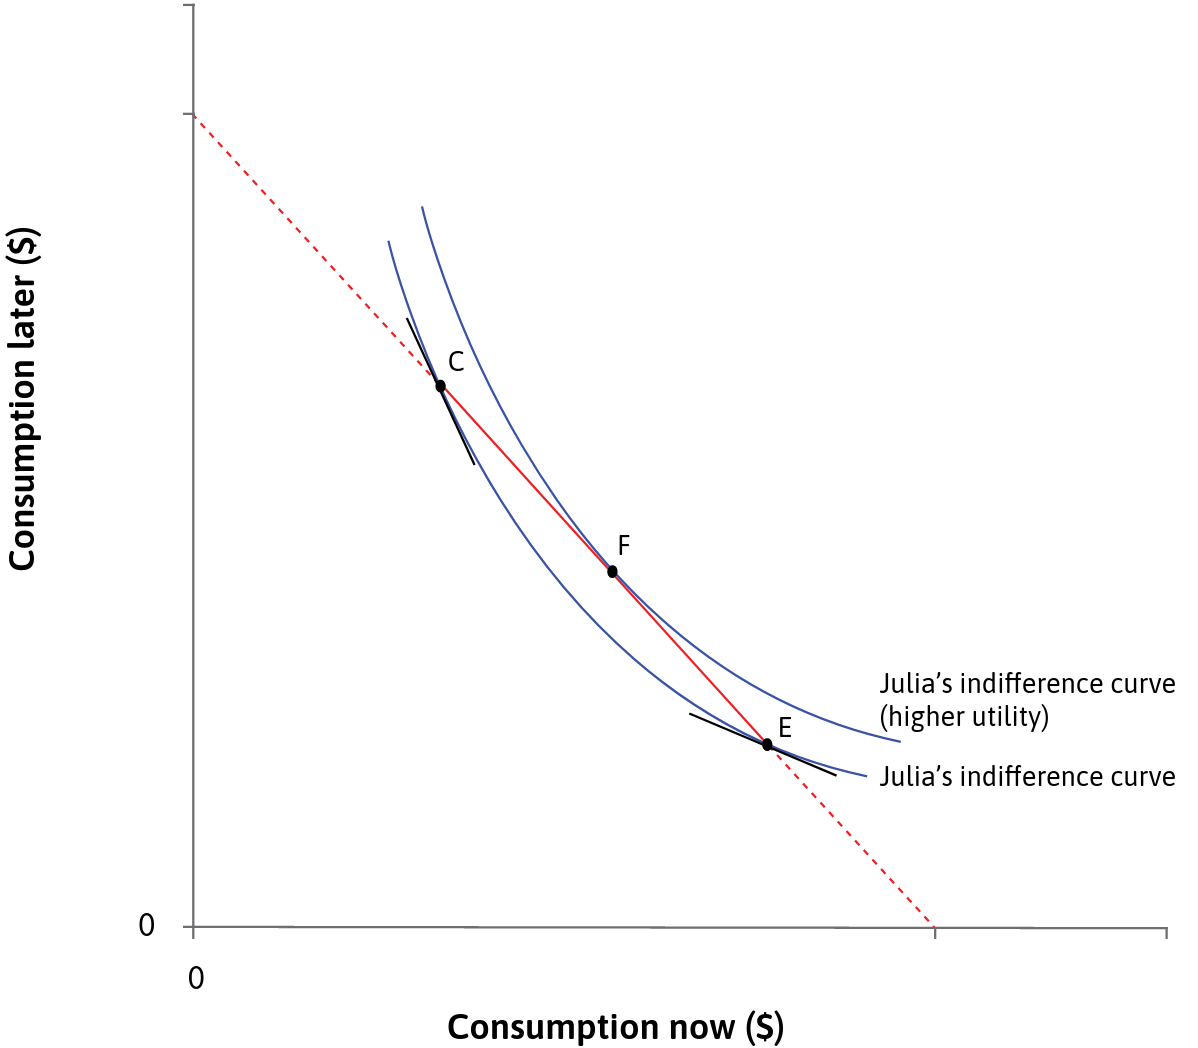
\includegraphics[width=\textwidth]{./figures/Figure3.png}
            \end{figure}

        \end{column}
    \end{columns}
    <++>

\end{frame}
<++>

\section{Appendix}
\label{sec:Appendix}

\appendix
% -------------------------------------------
\setbeamertemplate{headline}
{
\setbeamercolor{section in head/foot}{fg=black, bg=white}
\vskip1em \tiny \insertsectionnavigationhorizontal{1\paperwidth}{\hspace{0.50\paperwidth}}{}
}
%------------------------------------------
% \begin{frame}\frametitle{}
% \begin{columns}
% \label{Appendix}
% \column{1\linewidth}
% \centering
% {\Large \alert{Appendix}}
% \end{columns}
% \end{frame}
%------------------------------------------
\begin{frame}[allowframebreaks]{References}
\footnotesize
\bibliographystyle{$BIB_STYLE}
\bibliography{$BIBFILE}
\end{frame}

\end{document}
